\documentclass{article}
 

 
\usepackage[margin=1in]{geometry} 
\usepackage{amsmath,amsthm,amssymb}
 \usepackage{graphicx}
 \usepackage{enumerate}
 \usepackage{color}
 \usepackage{hyperref}
 
 \hypersetup{urlcolor=cyan}
 
\newcommand{\N}{\mathbb{N}}
\newcommand{\Z}{\mathbb{Z}}

\newcommand\numberthis{\addtocounter{equation}{1}\tag{\theequation}}

\def\R{\mathbb{R}}
\def\Zp{\mathbb{Z}^+}

\def\a{\alpha}
\def\b{\beta}
\def\c{\gamma}

 
\begin{document}
 
% --------------------------------------------------------------
%                         Start here
% --------------------------------------------------------------
 
 
%%%%%%%%%%%%%%%%%%%%%%%%%%%%%%%%%
% TITLE PAGE
%%%%%%%%%%%%%%%%%%%%%%%%%%%%%%%%% 
\title{
    \textmd{\Huge{Midterm A1}}\\
    \textmd{\huge{Section 4}}
}


\maketitle

Consider the set of points $(-2, 2)$, $(0, 1)$ and $(2, 2)$ and the interpolating polynomial $f(x)$, which is a $2^\text{nd}$ degree polynomial that passes through those points. \\

\textbf{Problem 1} [5pt]: If $f(x)$ is written as $\a x^2 + \b x + \c$, write down the linear system to be solved to obtain $\a$, $\b$ and $\c$. \\

Before anything, I do a quick sketch to see what's going on. \hspace*{3cm}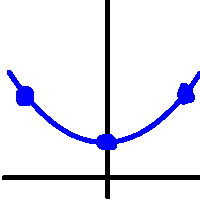
\includegraphics[scale=0.5]{thumbSketch}\\

Then I realize that this question is asking me to write down a system of equations, not find the scalar values $\a$, $\b$ and $\c$. Make note that these equations must be \textit{linear}. I have three points and an equation. There's only one thing I can do, really. What are three equations I can write with the given information? So I'm just going to plug each given $x$ value in and equate that with its $y$ value like this.

\begin{align*}
y_1 &= f(x_1) = \a x_1^2 + \b x_1 + \c \\
y_2 &= f(x_2) = \a x_2^2 + \b x_2 + \c \numberthis \\
y_3 &= f(x_3) = \a x_3^2 + \b x_3 + \c  \\
\end{align*}

Knowing that I'm looking for a linear system of equations, and knowing that \textit{linear system of equations} is a fancy way of saying \textit{matrix equation}, I'm going to rewrite it like this when I substitute the $(x_i, y_i)$'s back in. 

\begin{align*}
 \a (-2)^2 - \b 2 + \c &= 2 \\
 \a 0^2 + \b 0 + \c &= 1 \numberthis \\
 \a 2^2 + \b 2 + \c &= 2 \\
\end{align*}

If you weren't on facespace while the AMATH 301 lectures were playing dimly in the background, you'll probably recognize that (2) can be rewritten in fancy form like this.

\[
\begin{pmatrix} (-2)^2 & -2 & 1 \\ 0^2 & 0 & 1 \\ 2^2 & 2 & 1\\ \end{pmatrix}
\begin{pmatrix} \a \\ \b \\ \c \\ \end{pmatrix} = 
\begin{pmatrix} 2 \\ 1 \\ 2 \\ \end{pmatrix} \numberthis
\] 

And if you're really on your game, you can do this.

\[
\begin{pmatrix} 4 & -2 & 1 \\ 0 & 0 & 1 \\ 4 & 2 & 1\\ \end{pmatrix}
\begin{pmatrix} \a \\ \b \\ \c \\ \end{pmatrix} = 
\begin{pmatrix} 2 \\ 1 \\ 2 \\ \end{pmatrix} \numberthis
\] 

I awarded 5 points if you proved to me that you knew what you were doing. If you wrote down (2), (3), or (4), then you nailed it. Note that something along these lines 

\begin{align*}
y_1 &=  \a x_1^2 + \b x_1 + \c \\
y_2 &=  \a x_2^2 + \b x_2 + \c \\
y_3 &=  \a x_3^2 + \b x_3 + \c  \\
\end{align*}
\[
\text{where} \;\; \begin{pmatrix} x_1 \\ x_2 \\ x_3 \end{pmatrix} = \begin{pmatrix} -2 \\ 0 \\ 2 \end{pmatrix} \;\; \text{and} \;\; \begin{pmatrix} y_1 \\ y_2 \\ y_3 \end{pmatrix} = \begin{pmatrix} 2 \\ 1 \\ 2 \end{pmatrix}
\] \\

{\setlength{\parindent}{0cm}
would be a perfectly good answer because it would \textit{prove to me} that you know what you're doing. I'm surprised nobody tried that. Finally, I'd like to mention that if you don't \text{immediately} recognize the $3 \times 3$ matrix above as a Vandermonde matrix, go {\color{cyan} \underline{\href{http://en.wikipedia.org/wiki/Vandermonde_matrix}{here}}}. Notice that they mention that "some authors use the transpose." Other authors (like ours) do it differently.}\\

\textbf{Problem 2} [10pt]: The system above can be row-reduced to the following system:

\[
\begin{pmatrix} 4 & -2 & 1 \\ 0 & 4 & 0 \\ 0 & 0 & 1 \end{pmatrix} \begin{pmatrix} \a \\ \b \\ \c \end{pmatrix} = \begin{pmatrix} 2 \\ 0 \\ 1 \end{pmatrix}
\]

Solve this system for $\a$, $\b$, and $\c$.\\

When all else fails, just play with the given information. Get it into a new form. Sometimes it helps to look at things in a different light. We can matrix-multiply the equation above to get


\begin{align*}
4 \a - 2 \b + \c &= 2 \\
4 \b &= 0 \\
\c & = 1
\end{align*}

\textbf{Stop!} What does $4 \b = 0$ mean? Well, if you take 4, multiply it by something and get 0, that something \textit{must} be 0. So the equation $4 \b = 0$ implies $\b = 0$. Always be on the lookout for zeros; they (usually) make things a lot easier. From here, we see that since $\b = 0$ and $\c = 1$, we can substitute into the first equation to get

\begin{align*}
4 \a - 2 \b + \c &= 2 \\
4 \a - 2 (0) + 1 &= 2 \\
4 \a &= 1 \\
\a &= \frac{1}{4}
\end{align*}

You could have done this with the powerful tools of linear algebra (i.e. row operations, back substitution, \dots ), but these tools are a bit \textit{too} powerful for this problem. Notice that the $3 \times 3$ matrix is $44.444\dots$\% zeros. Again, zeros are our friends in this case. If you understand that a matrix and a system of equations are \textit{\textbf{the same thing}}, then a quick glance at 

\[
\begin{pmatrix} 4 & -2 & 1 \\ 0 & 4 & 0 \\ 0 & 0 & 1 \end{pmatrix} \begin{pmatrix} \a \\ \b \\ \c \end{pmatrix} = \begin{pmatrix} 2 \\ 0 \\ 1 \end{pmatrix}
\]

{\setlength{\parindent}{0cm}
tells us that $\b = 0$ and $\c = 1$. From there you can do the rest in your head since the top row reduces nicely to $4 \a + 1 = 2$, so that $\a = 1/4$. If you were so inclined, you could just write
}

\[
\a = \frac{1}{4} \quad \b = 0 \quad \c = 1
\]

{\setlength{\parindent}{0cm}
but then I'd have no way of knowing if you happened to scribble that down in a last-ditch effort after looking at your buddy's answer. I need some kind of sign that you know what you're doing. Again, I tried to be fair. 
}



\end{document}











































